\chapter{Condizionamento dell'Ingresso}

%--------------------------------------------------------------------------------------------

\section{Convertitore Lineare-Esponenziale}

%--------------------------------------------------------------------------------------------

Vogliamo ora analizzare il circuto che soddisfa la specifica sulla modalità $1\ V/Octave$
dell'ingresso, ovvero il circuito in grado di convertire una tensione lineare in una
esponenziale.

La soluzione utilizzata è molto diffusa in questo tipo di applicazioni, si può infatti
trovare in molti siti di DIY come ad esempio quello di René Schmitz \cite{expo_converter},
personaggio molto noto tra gli appassionati di sintetizzatori musicali fai-da-te.

%--------------------------------------------------------------------------------------------

\subsection*{Analisi del Circuito}

%--------------------------------------------------------------------------------------------

Per l'applicazione si sfrutta la caratteristica esponenziale intrinseca del transistor
bipolare, ovvero:

\begin{equation}\label{transistor_current}
    I_e\approx I_c=I_se^{\left(\frac{V_{be}}{V_T}-1\right)}
    \approx I_se^{\left(\frac{V_{be}}{V_T}\right)}\ [A]
\end{equation}

\begin{figure}[H]
    \centering
    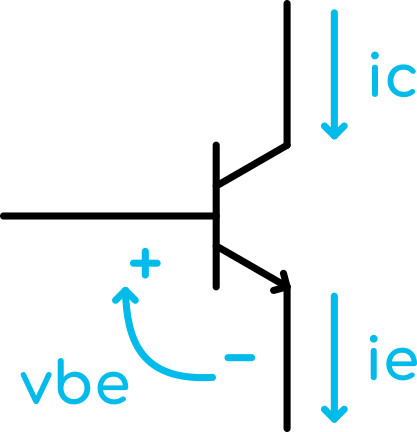
\includegraphics{circuits/single_transistor_circuit.png}
    \caption{BJT}
    \label{bjt}
\end{figure}

dove $V_T$ (potenziale termico) e $I_s$ (corrente di saturazione) sono variabili in
funzione della temperatura. Nella nostra analisi $V_T$ verrà considerato di valore costante
pari a $26\ mV$, mentre si rimuove dall'equazione $I_s$ collegando una coppia di transistor
(idealmente nello stesso chip, in modo che siano il più possibile simili tra loro e
termicamente accoppiati) in configurazione differenziale:

\begin{figure}[H]
    \centering
    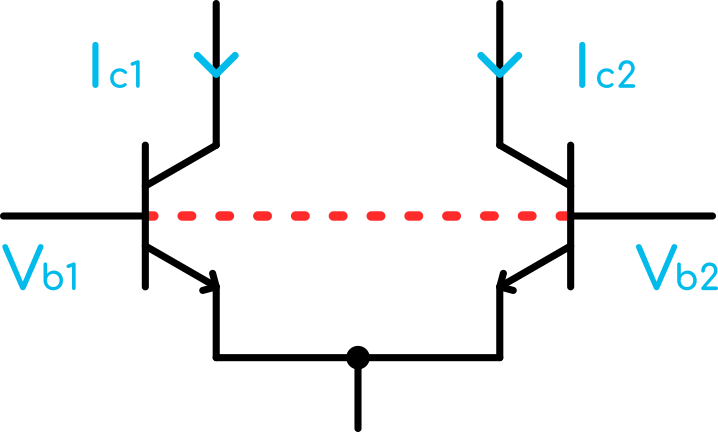
\includegraphics{circuits/differential_pair_circuit.png}
    \caption{BJT a coppia differenziale}
    \label{differential_pair_circuit}
\end{figure}

in questo modo possiamo scrivere la seguente relazione:

\begin{equation}\label{differential_pair}
    \frac{I_{c2}}{I_{c1}}=\frac{I_s e^{\left(\frac{V_{be2}}{V_T}\right)}}{I_s e^{\left(\frac{V_{be1}}{V_T}\right)}}
    \qquad
    \rightarrow
    \qquad
    I_{c2}=I_{c1}e^{\left(\frac{V_{be2}-V_{be1}}{V_T}\right)}=I_{c1}e^{\left(\frac{V_{b2}-V_{b1}}{V_T}\right)}\ [A]
\end{equation}

dove risulta evidente che la dipendenza da $I_s$ viene completamente rimossa.

A questo punto, rinominiamo le grandezze come segue:

\begin{equation}\label{renamed_differential_pair}
    \left\{ \begin{aligned}
        I_{c2} & = I_{freq} \\
        I_{c2} & = I_{ref}
    \end{aligned} \right.
    \qquad
    \rightarrow
    \qquad
    I_{freq}=I_{ref}e^{\left(\frac{V_{b2}-V_{b1}}{V_T}\right)}\ [A]
\end{equation}

e aggiungiamo al circuito

\begin{itemize}
    \item un amplificatore invertente per portare $V_{in}$ in un range appropriato alla base
          di $Q_1$ (operazionale di sinistra, figura \ref{exponential_converter_circuit})
          \begin{equation}\label{amplifier}
              V_{b1}=-V_{in}\cdot s=
              -V_{in}\cdot\frac{R_f}{R_{in}}\cdot\frac{\%R_{pot}+R}{R_{pot}+R}\ [V]
          \end{equation}
    \item un anello di controllo per mantenere la corrente di riferimento $I_{ref}$ costante
          (operazionale centrale, figura \ref{exponential_converter_circuit})
          \begin{equation}\label{iref}
              I_{ref}=\frac{V_{HR}-V_{LR}}{R_{ref}}\ [A]
          \end{equation}
    \item un convertitore corrente-tensione al collettore di $Q_2$ (operazionale di destra,
          figura \ref{exponential_converter_circuit})
          \begin{equation}\label{ivconv}
              V_{exp}=I_{freq}\cdot R_{conv}\ [V]
          \end{equation}
\end{itemize}

ottenendo quindi il seguente circuito con la relativa relazione ingresso/uscita:

\begin{figure}[H]
    \centering
    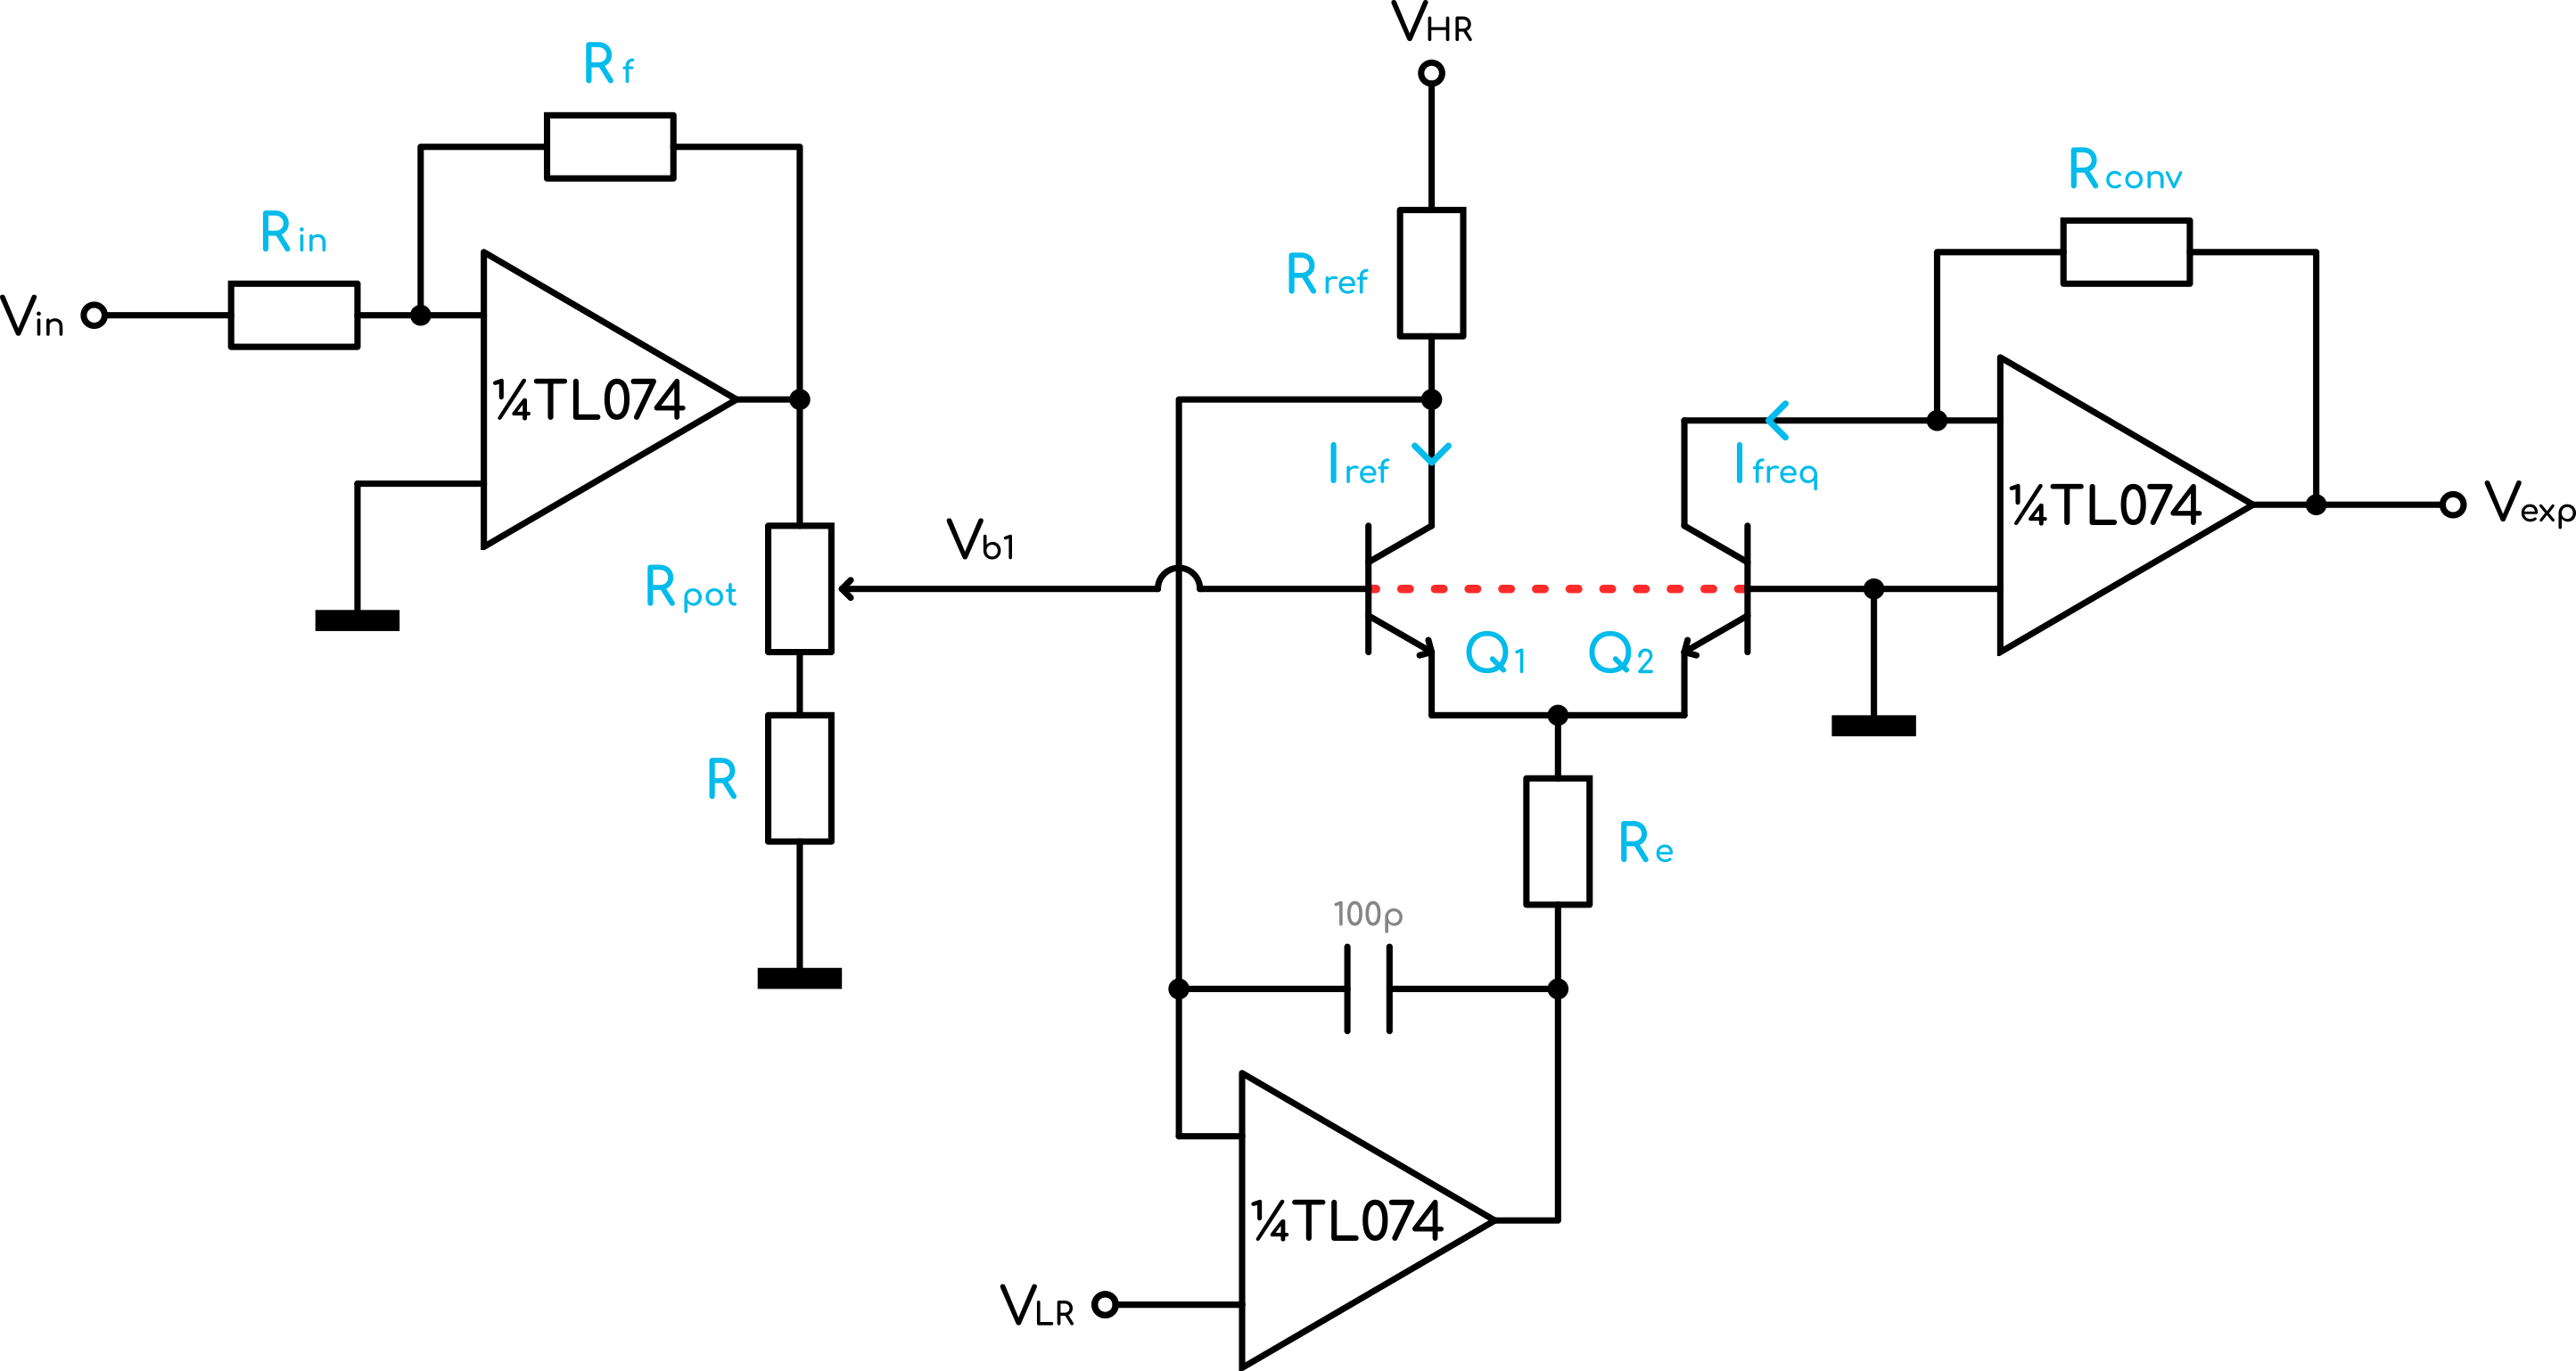
\includegraphics{circuits/exponential_converter_circuit.png}
    \caption{Schema elettrico del convertitore tensione lineare-esponenziale}
    \label{exponential_converter_circuit}
\end{figure}

\begin{equation}\label{expo_converter}
    V_{exp}=R_{conv}\cdot \frac{V_{HR}-V_{LR}}{R_{ref}}e^{\left(\frac{s\cdot V_{in}}{V_T}\right)}\ [V]
\end{equation}

%--------------------------------------------------------------------------------------------

\subsection*{Dimensionamento e Scelta dei Componenti}

%--------------------------------------------------------------------------------------------

Passiamo quindi al dimensionamento dei componenti, in modo da imporre al circuito il
comportamento voluto.

Come prima cosa calcoliamo il valore del guadagno $s$ dell'amplificatore invertente.
Si vuole:

\begin{equation}\label{iref_doubling}
    I_{freq}=I_{ref}e^{\left(\frac{s\cdot V_{in}}{V_T}\right)}
    \qquad
    \xrightarrow{+\Delta V_{in}}
    \qquad
    2I_{freq}=I_{ref}e^{\left(\frac{s\cdot(V_{in}+\Delta V_{in})}{V_T}\right)}
\end{equation}

qundi un raddoppio della corrente $I_{freq}$ per ogni variazione $\Delta V_{in}=1\ V$.
Allora possiamo riscrivere la relazione nel seguente modo:

\begin{equation}\label{s1}
    \frac{2I_{freq}}{I_{freq}}=
    \frac{I_{ref}e^{\left(\frac{s\cdot(V_{in}+\Delta V_{in})}{V_T}\right)}}
    {I_{ref}e^{\left(\frac{s\cdot V_{in}}{V_T}\right)}}
    \
    \rightarrow
    \
    2=e^{\left(\frac{s\cdot\Delta V_{in}}{V_T}\right)}
    \
    \rightarrow
    \
    ln(2)=\frac{s\cdot\Delta V_{in}}{V_T}
    \
    \rightarrow
    \
    s=\frac{V_T\cdot ln(2)}{\Delta V_{in}}
\end{equation}

\begin{equation}\label{s2}
    s=\frac{26\ mV\cdot 0.6931}{1\ V}\approx0.018\approx\frac{1}{55.5}
\end{equation}

\begin{equation}\label{s3}
    s=\frac{R_f}{R_{in}}\cdot\frac{\%R_{pot}+R}{R_{pot}+R}
    =\frac{2\ k\Omega}{100\ k\Omega}\cdot\frac{440\ \Omega}{490\ \Omega}
    \approx 0.018
\end{equation}

quindi:

\begin{itemize}
    \item $R_f = 2\ k\Omega$;
    \item $R_{in} = 100\ k\Omega$;
    \item $R_{pot} = 100\ \Omega$;
    \item $R = 390\ \Omega$;
\end{itemize}

Scegliamo poi $R_{conv}=3.3\ k\Omega$, per avere come massimo valore di corrente
$I_{freq} = 3\ mA$ (ovvero $V_{exp}\approx+10\ V$ in uscita dal convertitore corrente-tensione),
in corrispondenza di una tensione di ingresso $V_{in}=+8\ V$. Da qui possiamo calcolare il
valore di $I_{ref}$:

\begin{equation}\label{iref_calc}
    I_{ref}=I_{freq}e^{\left(-\frac{s\cdot V_{in}}{V_T}\right)}
    =0.003e^{\left(-\frac{0.018\cdot8}{0.026}\right)}
    \approx11.8\ \mu A
\end{equation}

Poi impostando $V_{HR}=+12\ V$ e $V_{LR}=0\ V$ calcoliamo $R_{ref}$:

\begin{equation}\label{rref_calc}
    R_{ref}=\frac{V_{HR}}{I_{ref}}=\frac{12}{11.8\cdot10^{-6}}\approx 1\ M\Omega
\end{equation}

La scelta di $R_e$ sarebbe ora condizionata dalla tensione di saturazione dell'operazionale,
poichè altrimenti il circuito smetterebbe di comportarsi come desiderato, cambiando il
riferimento di $V_{LR}$ e quindi anche $I_{ref}$. Avendo collegato la base di $Q_2$ a massa
il potenziale agli emettitori dovrà rimanere costante a circa $-V_{be}$ per qualsiasi valore
di tensione in ingresso, quindi la tensione in uscita dall'operazionale avrà valore

\begin{equation}
    V_{op}=-V_{be}-R_e(I_{c1}+I_{c2})=%
    -V_{be}-R_e\cdot I_{ref}\left(1+e^{\left(\frac{sV_{in}}{V_T}\right)}\right)\ [V]
\end{equation}

che assumerà il valore massimo a $V_{in}=+8\ V$, con una corrente di circa $3\ mA$  in $R_e$.
Volendo imporre una tensione di saturazione di valore $-V_{sat}=-10.5\ V$ calcoliamo il valore
di $R_e$.

\begin{equation}
    R_e=\frac{V_{op}+V_{be}}{-I_{ref}\left(1+e^{\left(\frac{sV_{in}}{V_T}\right)}\right)}=
    \frac{-10.5+0.7}{-12\cdot10^{-6}\left(1+e^{\left(\frac{0.018\cdot8}{0.026}\right)}\right)}=
    \frac{9.8}{0.003}\approx 3.3\ k\Omega
\end{equation}

Se però andiamo a calcolare la caduta di potenziale ai capi di $R_e$ corrispondente a $V_{in}=0\ V$,
ovvero:

\begin{equation}\label{vre}
    V_{R_e}=2R_e\cdot I_{ref}=3.3\cdot10^3\cdot24\cdot10^{-6}\approx79.2\ mV
\end{equation}

notiamo che un valore di resistenza maggiore aumenterebbe la linearità del circuito per bassi
livelli di $V_{in}$, in quanto incrementerebbe la caduta di potenziale sul resistore,
risultando quindi meno influenzata dal rumore. Si modifica allora il circuito cosicché la
resistenza di emettitore sia variabile in modo non-lineare, a seconda della corrente richiesta
in uscita. Questo è reso possibile sostituendo ad $R_e$ un parallelo tra due resistori di
diverso valore, di cui quello più piccolo collegato in serie ad un diodo, l'elemento che si
occuperà effettivamente di modificare il valore di resistenza.

\begin{figure}[H]
    \centering
    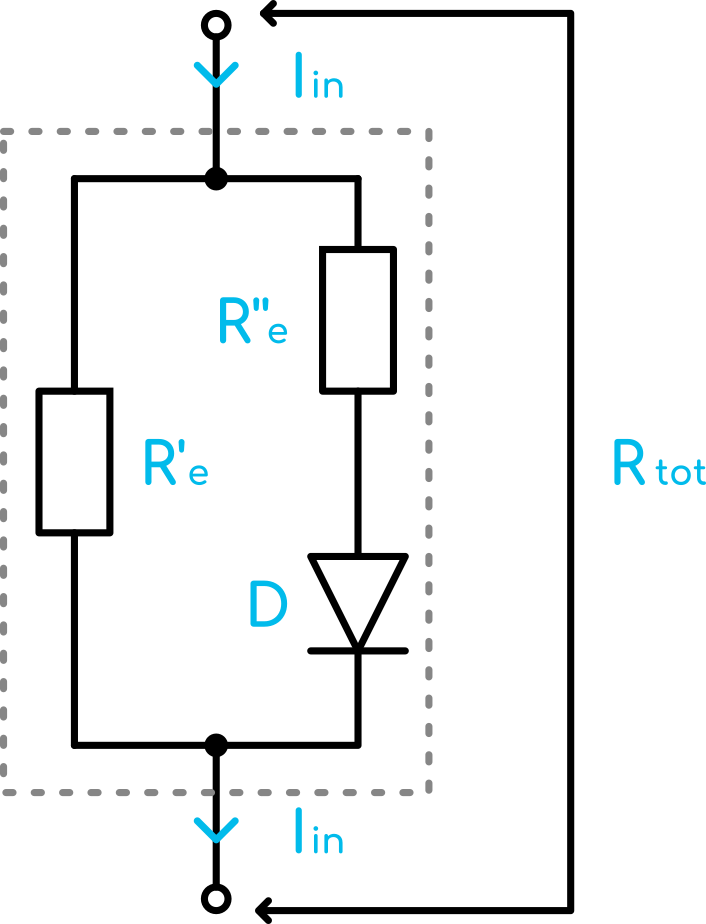
\includegraphics{circuits/Rtot_circuit.png}
    \caption{Schema elettrico del resistore di emettitore equivalente}
    \label{Rtot_circuit}
\end{figure}

Si scelgono $R_e'=10\ k\Omega$ e $R_e''=1.2\ k\Omega$.

\begin{equation}\label{rtot}
    R_{tot} =
    \left\{
    \begin{array}{lr}
        R_e'        & \text{con diodo spento, ovvero } I_{ref}+I_{freq}\leq\frac{V_d}{R_e'} \\
        R_e'//R_e'' & \text{con diodo acceso, ovvero } I_{ref}+I_{freq}>\frac{V_d}{R_e'}
    \end{array}
    \right.
\end{equation}

Per quanto riguarda i componenti, ancora una volta gli amplificatori operazionali utilizzati
sono dei TL074, mentre si sceglie un MPQ3904 \cite{mpq3904} per i transistor, chip che
ospita 4 unità molto simili tra loro e termicamente accoppiati, e vista la disponibilità, il
diodo viene sostituito con uno dei 4 transistor del chip configurato come diodo, quindi
collegando base e collettore assieme.

\begin{figure}[H]
    \centering
    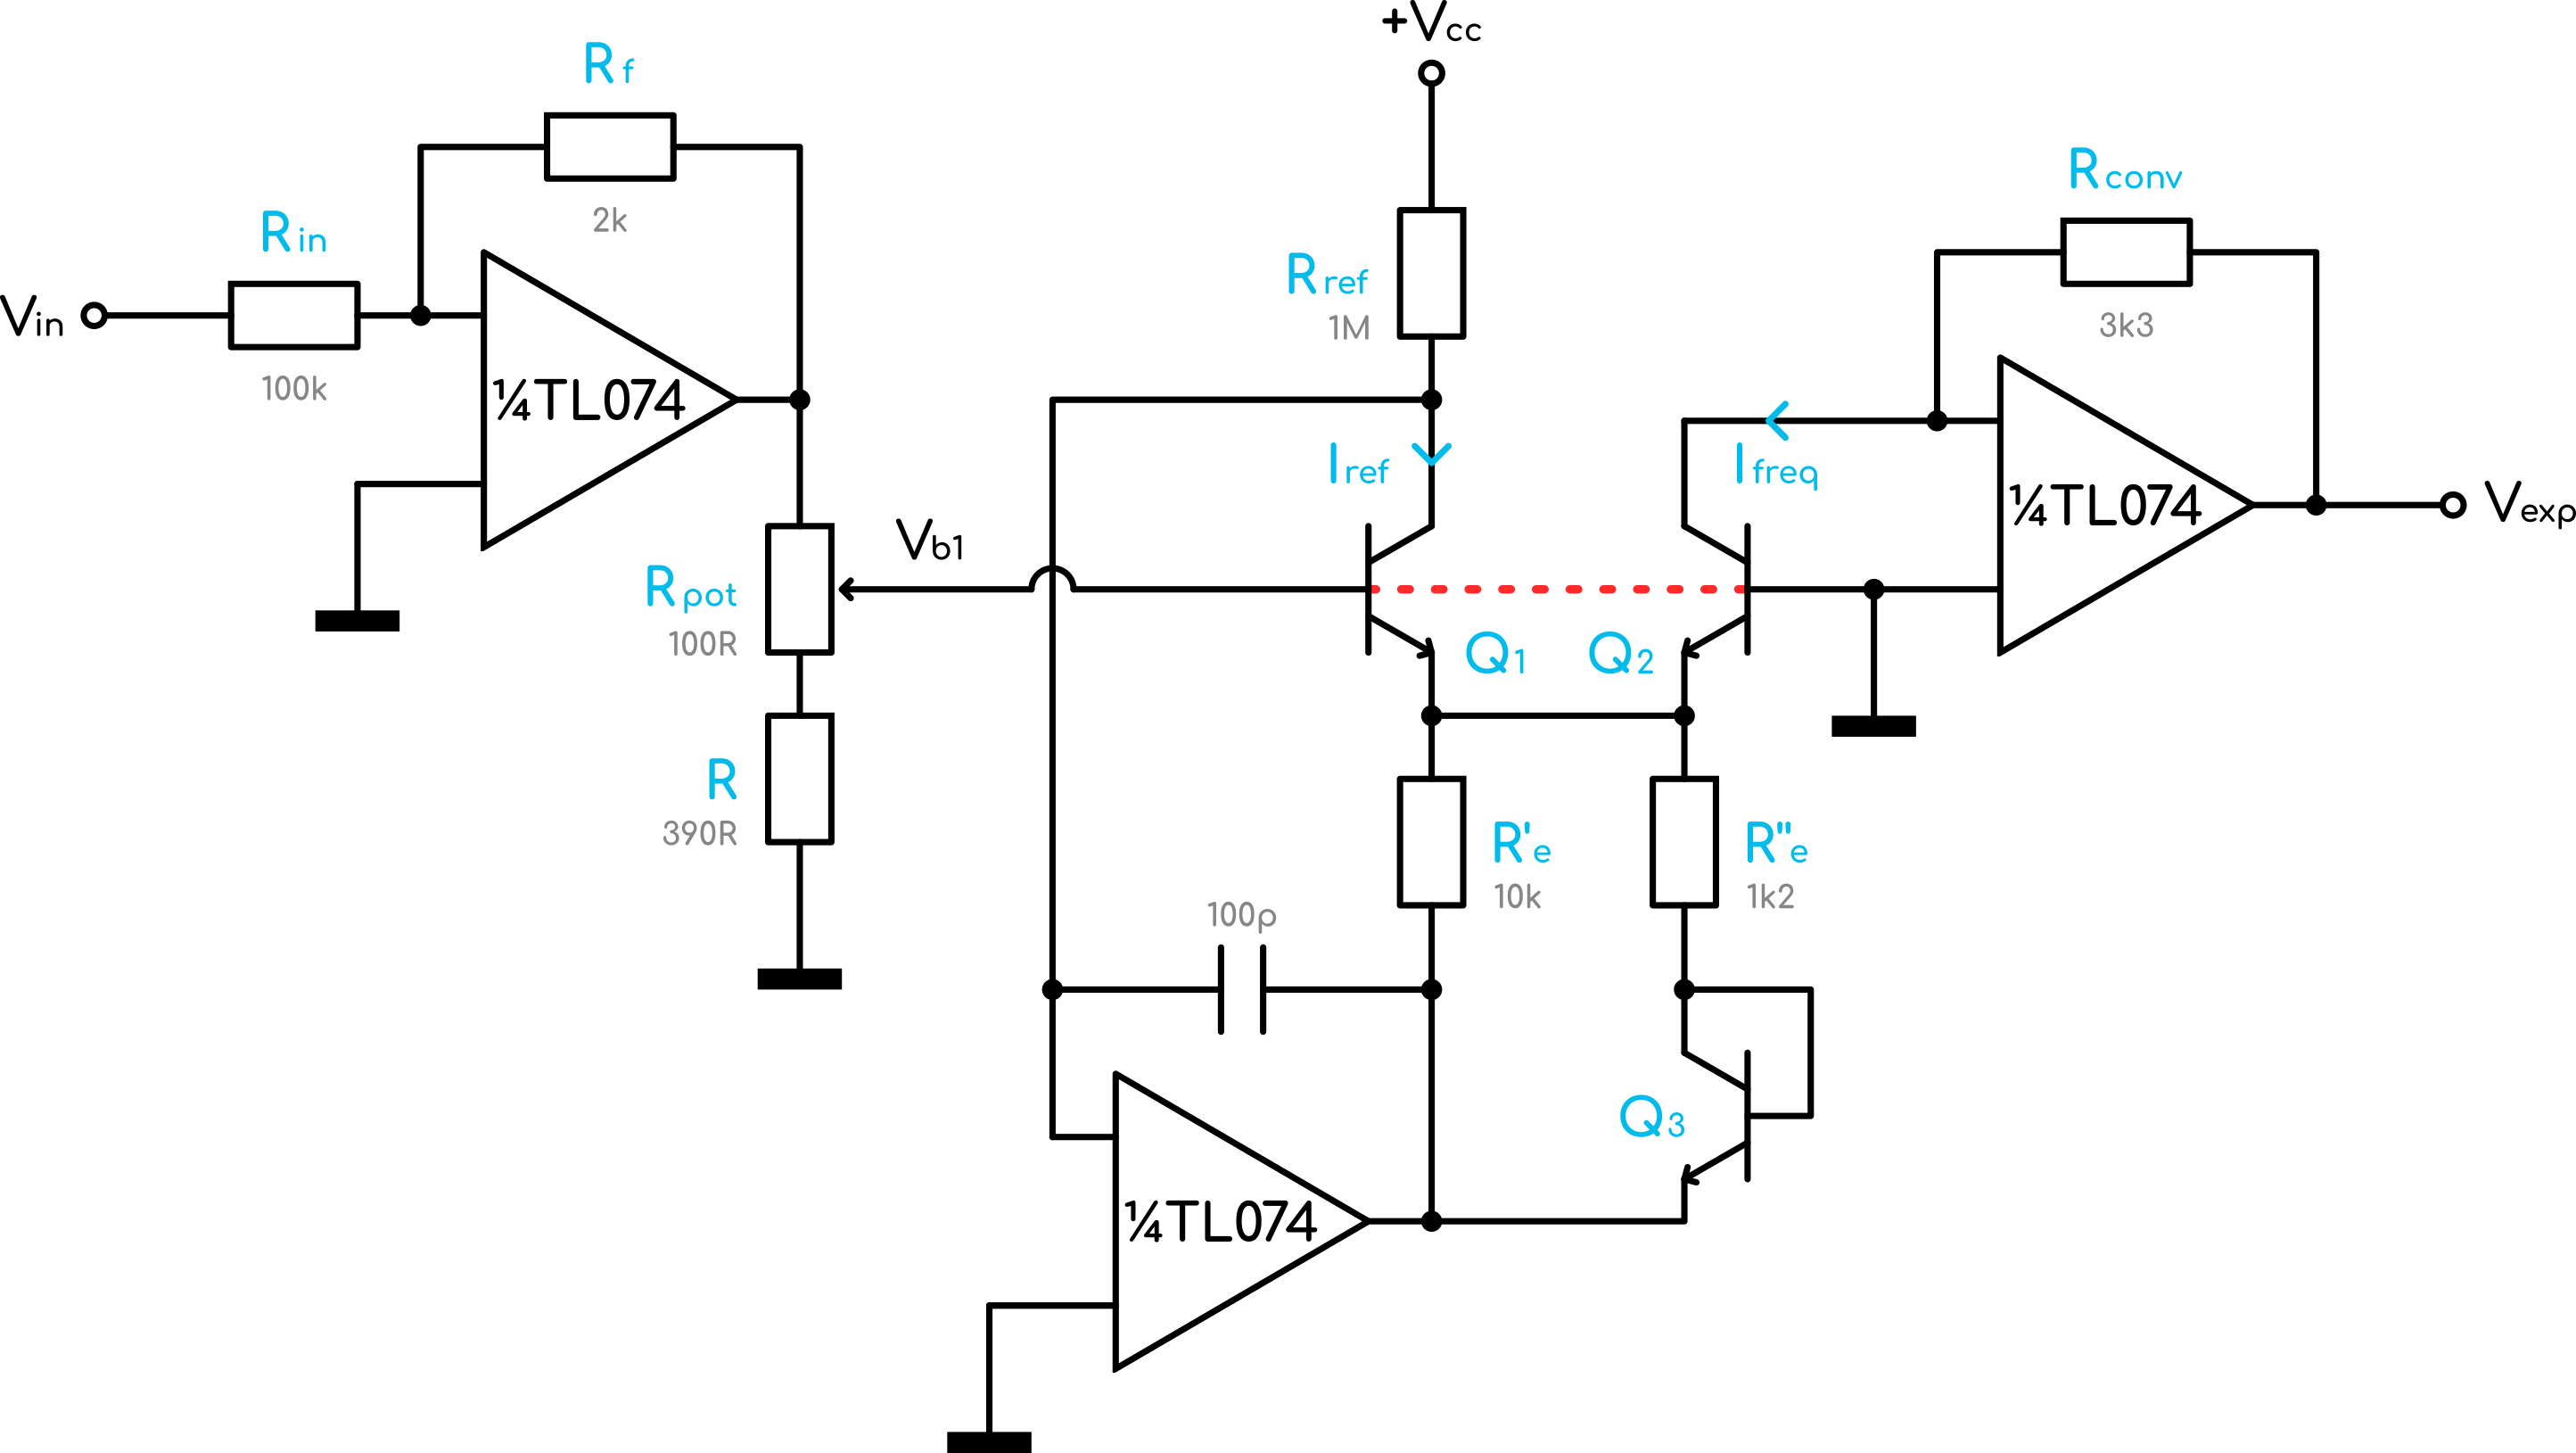
\includegraphics{circuits/complete_exponential_converter_circuit.png}
    \caption{Schema elettrico completo del convertitore tensione lineare-esponenziale ($+V_{cc}=+12\ V$)}
    \label{complete_exponential_converter_circuit}
\end{figure}

%--------------------------------------------------------------------------------------------

\subsection*{Risultati Pratici e Misure}

%--------------------------------------------------------------------------------------------

Analizziamo ora il comportamento del circuito.

\begin{figure}[H]
    \centering

    \begin{subfigure}{.5\textwidth}
        \centering
        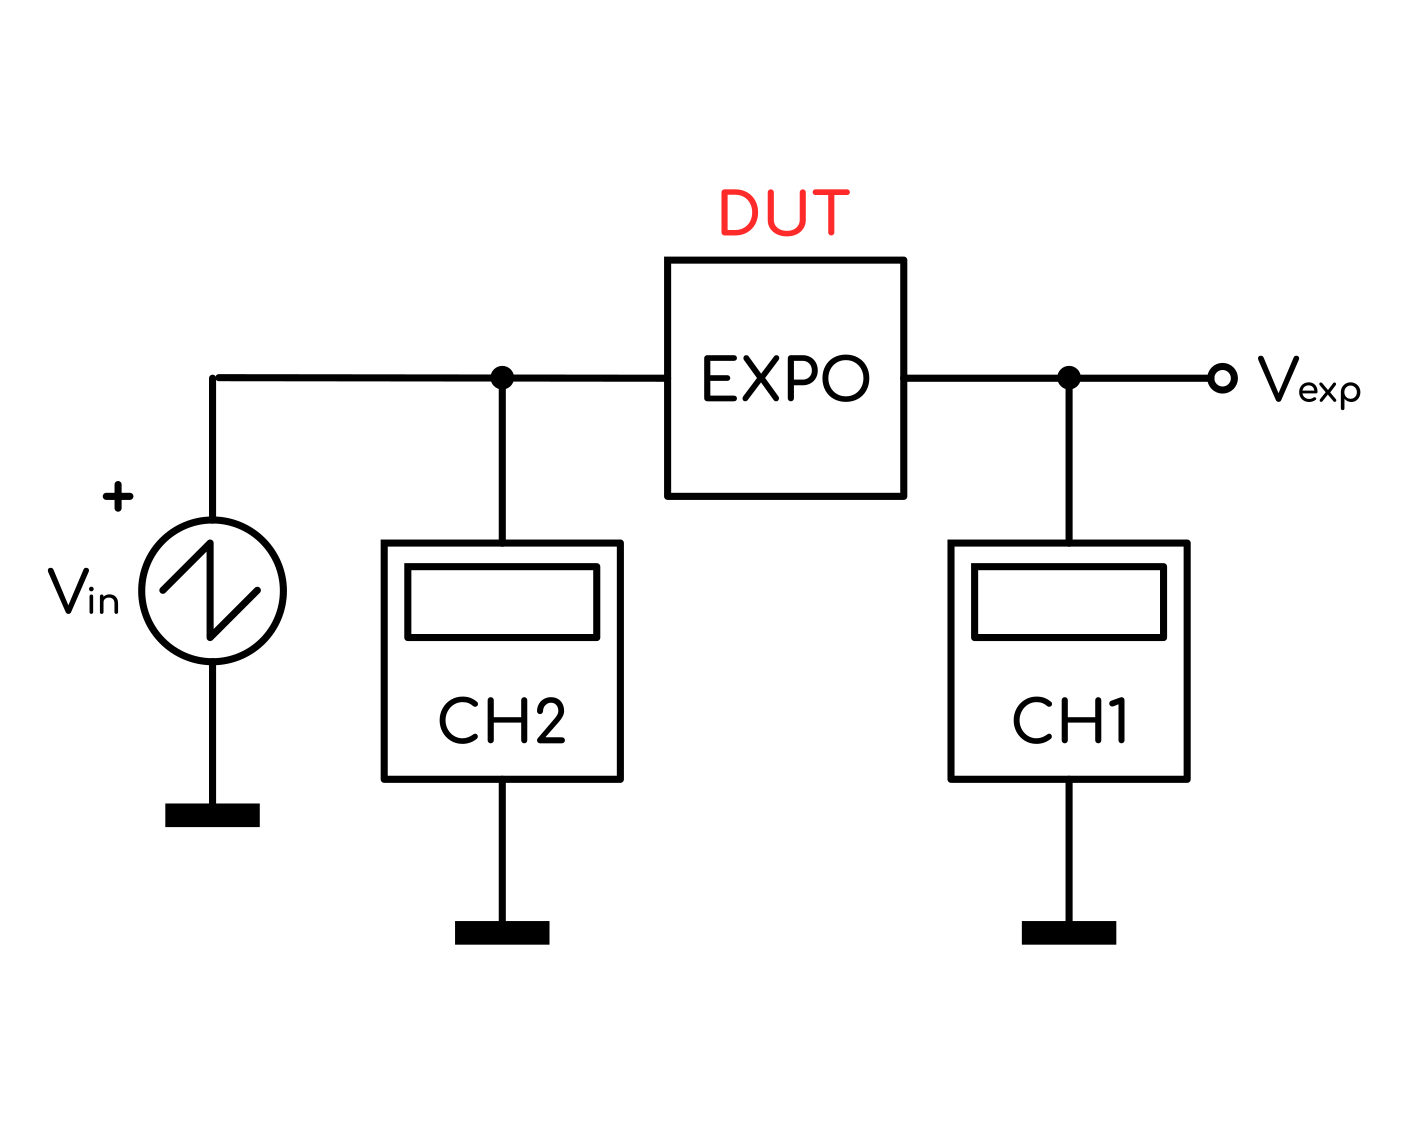
\includegraphics{block_diagrams/mis_expo_oscilloscope.png}
        \caption{Setup di misura}
        \label{mis_expo_oscilloscope}
    \end{subfigure}%
    \begin{subfigure}{.5\textwidth}
        \centering
        
\includegraphics{misc/oscilloscope_placeholder.png}
        \caption{Transcaratteristica}
        \label{expo_transcharacteristic}
    \end{subfigure}

    \caption{Misura della transcaratteristica con oscilloscopio}
\end{figure}

\begin{minipage}{0.49\textwidth}
    \centering
    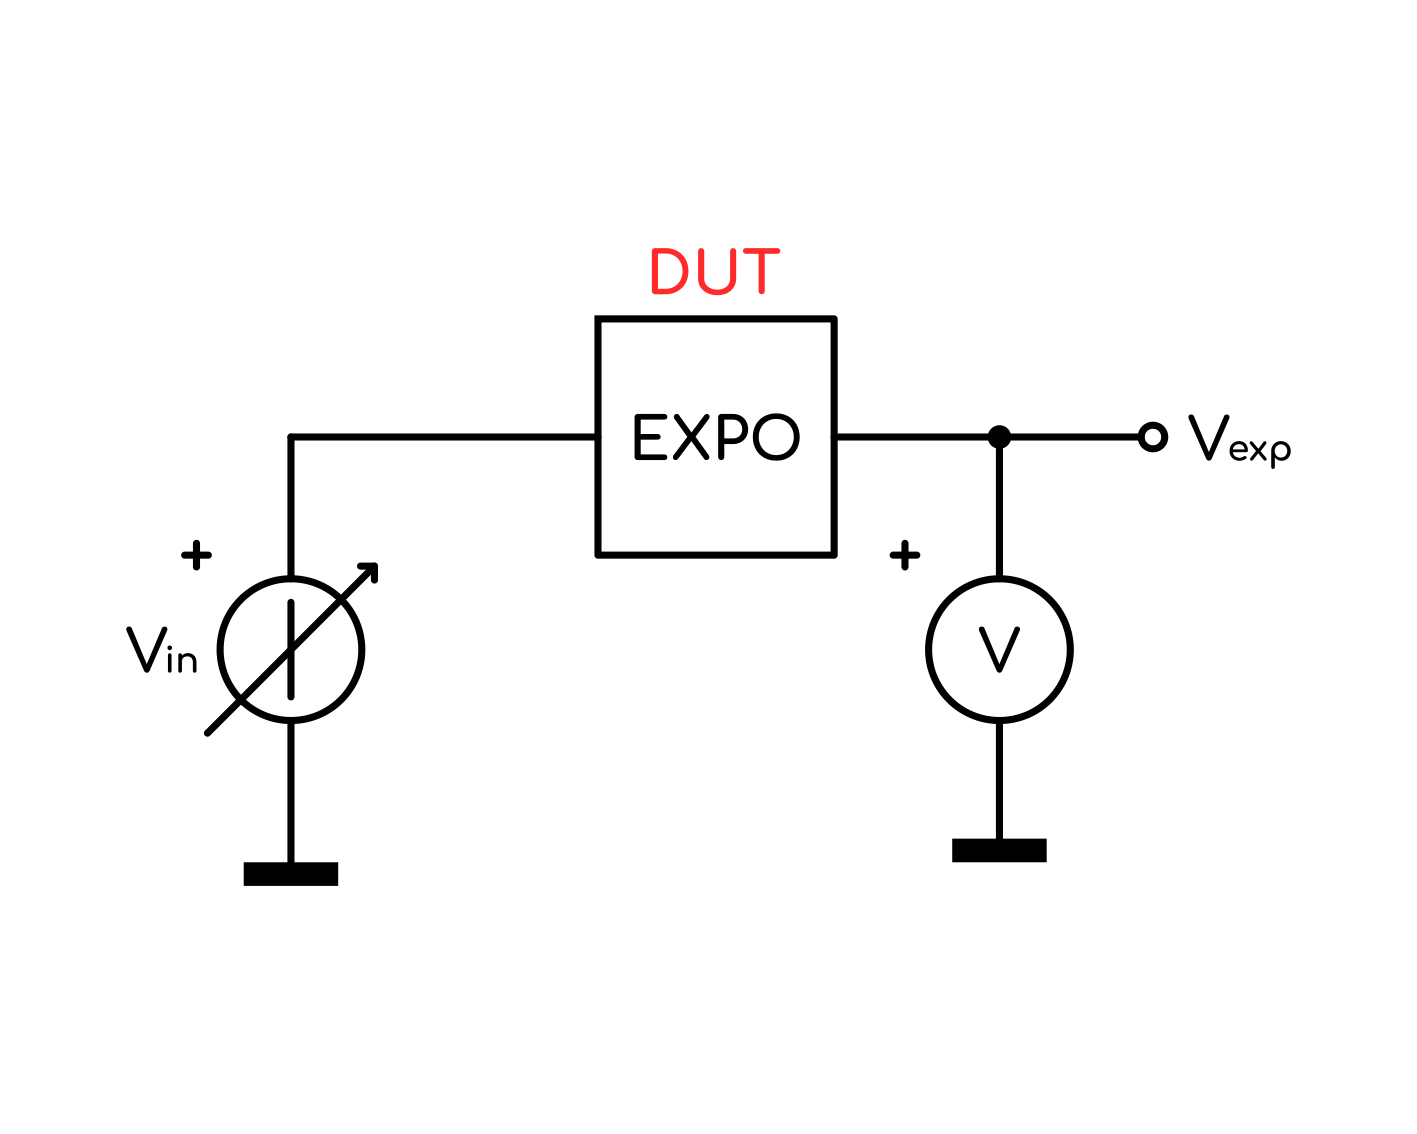
\includegraphics{block_diagrams/mis_expo.png}
    \captionof{figure}{Setup di misura}
    \label{mis_expo}
\end{minipage}
\begin{minipage}{0.49\textwidth}
    \centering
    \begin{table}[H]
        \centering
        \csvreader[
        tabular = |C||C|L|,
        table head = {\hline \rowcolor{myLightGrey} $V_{in}\ [V]$ & $V_{exp}\ [V]$ & $2^{V_{in}}\ [V]$ \\\hline},
        late after line = \\\hline,
        ]{data/misure_expo.csv}{}{
        \csvcoli & \csvcoliii & \csvcolii
        }
        \caption{Valori misurati}
        \label{expo_table}
    \end{table}
\end{minipage}

\begin{figure}[H]
    \centering

    \begin{subfigure}{.5\textwidth}
        \centering
        \begin{tikzpicture}[scale = 0.85]
            \begin{semilogyaxis}[
                    title = Transcaratteristica in scala logaritmica,
                    no marks,
                    xmin = 0, xmax = 12,
                    ymin = 0.01, ymax = 100,
                    grid = major,
                    grid style = {dashed, gray!30},
                    xlabel = $V_{in}$,
                    ylabel = $V_{exp}$,
                    x unit = \si{\V}, y unit = \si{\V},
                    legend style = {at = {(0.5, -0.25)}, anchor = north},
                    cycle list name = modular,
                ]

                \addplot
                table[x = vin, y = vexp formula, col sep = comma]{./data/misure_expo.csv};

                \addplot
                table[x = vin, y = vexp attesa, col sep = comma]{./data/misure_expo.csv};

                \addplot
                table[x = vin, y = vexp misura, col sep = comma]{./data/misure_expo.csv};

                \legend{Formula \ref{expo_converter}, Valori attesi, Valori misurati}
            \end{semilogyaxis}
        \end{tikzpicture}
    \end{subfigure}%
    \begin{subfigure}{.5\textwidth}
        \centering
        \begin{tikzpicture}[scale = 0.85]
            \begin{axis}[
                    title = Transcaratteristica in scala lineare,
                    no marks,
                    xmin = 0, xmax = 12,
                    ymin = 0, ymax = 15,
                    grid = major,
                    grid style = {dashed, gray!30},
                    xlabel = $V_{in}$,
                    ylabel = $V_{exp}$,
                    x unit = \si{\V}, y unit = \si{\V},
                    legend style = {at = {(0.5, -0.25)}, anchor = north},
                    cycle list name = modular,
                ]

                \addplot
                table[x = vin, y = vexp formula, col sep = comma]{./data/misure_expo.csv};

                \addplot
                table[x = vin, y = vexp attesa, col sep = comma]{./data/misure_expo.csv};

                \addplot
                table[x = vin, y = vexp misura, col sep = comma]{./data/misure_expo.csv};

                \legend{Formula \ref{expo_converter}, Valori attesi, Valori misurati}
            \end{axis}
        \end{tikzpicture}
    \end{subfigure}

    \caption{Grafici delle misure riportate in tabella \ref{expo_table}}
    \label{expo_graphs}
\end{figure}

In azzurro possiamo vedere i valori calcolati tramite la formula \ref{expo_converter},
in rosso invece i valori ottenuti moltiplicando il dato misurato a $0\ V$ per $2^{V_{in}}$
e infine in nero i valori effettivamente misurati. Si vede che rispetto a quanto calcolato
c'è un lieve discostamento dovuto con ogni probabilità alla tolleranza dei valori dei
componenti utilizzati, tuttavia le misure risultano quasi coincidenti con la curva esponenziale
di pendenza $2$ (in rosso), quindi possiamo affermare che il circuito funziona come desiderato.

Il ginocchio presente subito dopo i $10\ V$ è dovuto alla saturazione dell'operazionale
nel convertitore corrente-tensione, che con una alimentazione di $\pm12\ V$ presenta dei
valori di saturazione di circa $\pm10.5\ V$.

Si verifica anche che la curva della transcaratteristica in scala lineare coincide con la
transcaratteristica tracciata con l'oscilloscopio (figura \ref{expo_transcharacteristic}).

%--------------------------------------------------------------------------------------------

\section{Somma di più Ingressi}

%--------------------------------------------------------------------------------------------

Per fare in modo che possa essere utilizzato un segnale in tensione come modulante (ingresso
LFO), si aggiunge un resistore uguale a $R_{in}$ all'ingresso invertente dell'amplificatore,
modificando quindi la relazione \ref{amplifier} nel seguente modo:

\begin{equation}
    V_{b1}=-s\cdot\sum_0^n{V_{n}}\ [V]
\end{equation}

\begin{figure}[H]
    \centering
    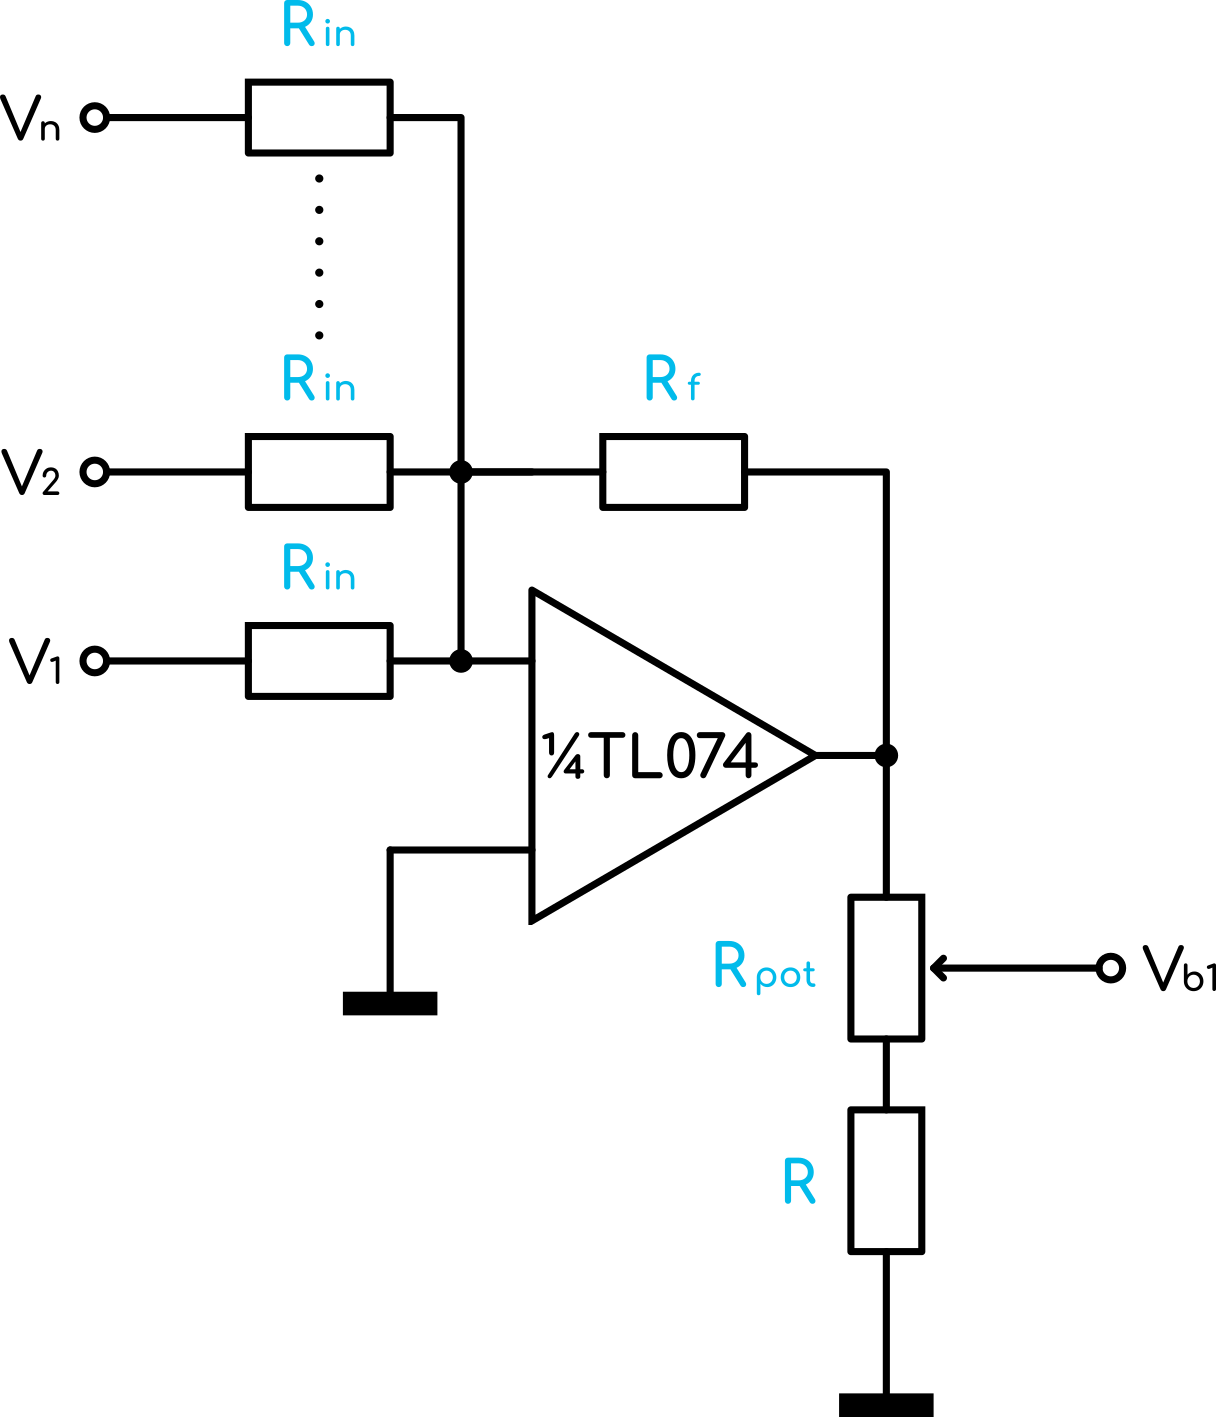
\includegraphics{circuits/summer_circuit.png}
    \caption{Circuito sommatore invertente}
    \label{summer_circuit}
\end{figure}

e rendendo quindi l'amplificatore un sommatore invertente. Si noti che non c'è un limite al
numero di ingressi che è possibile aggiungere.

Per la modulazione manuale si utilizzano due potenziometri, uno per una regolazione grossolana
e uno per una più fine, e li si collega ad uno degli ingressi del sommatore nel seguente modo:

\begin{figure}[H]
    \centering
    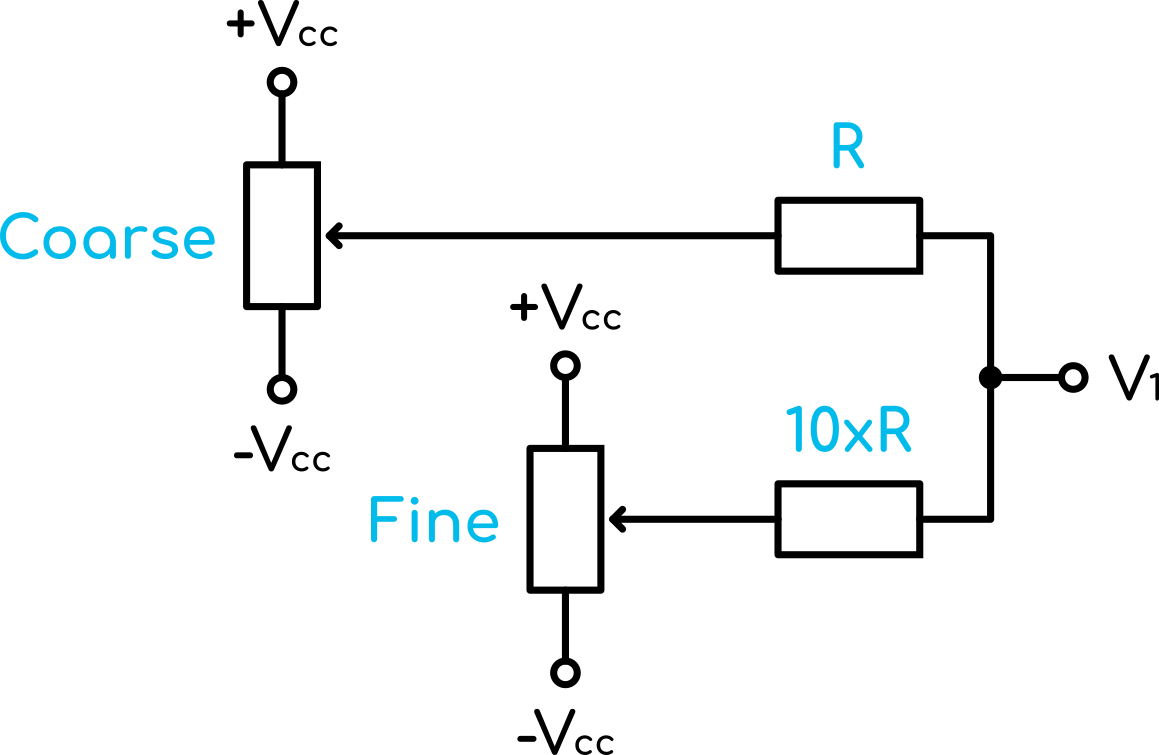
\includegraphics{circuits/coarse_fine_circuit.png}
    \caption{Circuito per la regolazione manuale della frequenza ($\pm V_{cc}=\pm12\ V$)}
    \label{coarse_fine_circuit}
\end{figure}

questo circuito permette di sommare (o sottrarre) una tensione compresa nel range di
alimentazione, inoltre la manopola "Fine" consente di regolare la tensione in modo più
preciso attorno al punto selezionato con "Coarse".

Infine, il segnale modulante d'ingresso viene portato ad un altro degli ingressi del sommatore,
attraverso un potenziometro per la regolazione del volume.

\begin{figure}[H]
    \centering
    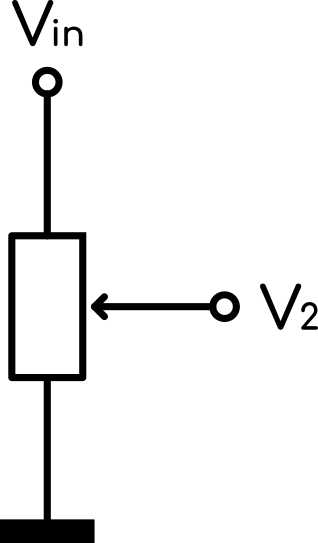
\includegraphics{circuits/lfo_input_circuit.png}
    \caption{Circuito di ingresso del segnale modulante}
    \label{lfo_input_circuit}
\end{figure}

%--------------------------------------------------------------------------------------------

\section{Raddrizzatore}

%--------------------------------------------------------------------------------------------

Come visto dalla formula \ref{expo_converter}, la tensione in ingresso $V_{in}$ deve essere di
valore positivo per polarizzare correttamente il transistor, e volendo inserire nel circuito
un nodo sommatore per avere la possibilità di utilizzare un segnale in tensione come modulante,
dobbiamo assicurarci che $V_{b1}$ non diventi mai positiva (il segno viene invertito
dall'amplificatore). Si aggiunge quindi un blocco raddrizzatore, realizzato con un diodo e
un operazionale, che compenserà per la caduta di tensione sul diodo. Lo schema utilizzato
è il seguente:

\begin{figure}[H]
    \centering
    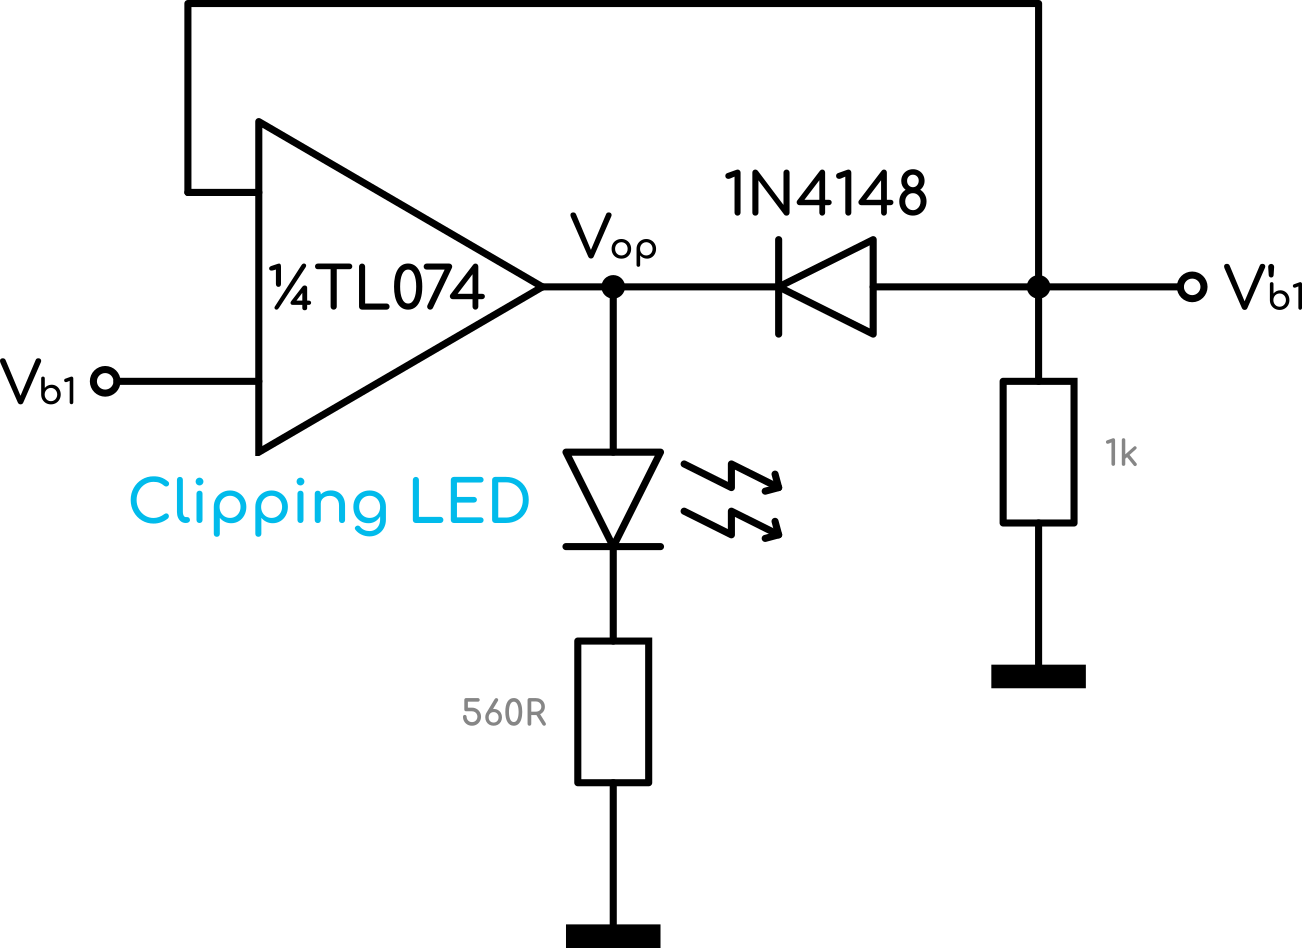
\includegraphics{circuits/clipper_circuit.png}
    \caption{Circuito raddrizzatore}
    \label{clipper_circuit}
\end{figure}

Il resistore collegato a $V_{b1}'$ è necessario per il ricircolo della corrente di
polarizzazione del diodo, che altrimenti non si accenderebbe mai. Viene inoltre aggiunto un
LED per visualizzare quando il raddrizzatore è in funzione, in modo da permettere all'utente
di correggere eventuali errori nel segnale modulante in ingresso.

Quindi in uscita si avrà la stessa tensione in ingresso se negativa, mentre un valore molto
prossimo a $0$ se positiva.

\begin{equation}\label{clipper_out}
    V_{out} =
    \left\{
    \begin{array}{lr}
        V_{in} & \text{con } V_{in}\le0 \\
        0      & \text{con } V_{in}>0
    \end{array}
    \right.
\end{equation}

\begin{equation}\label{clipper_op}
    V_{op} =
    \left\{
    \begin{array}{lr}
        V_{in}+V_d & \text{con } V_{in}\le0\Rightarrow \text{LED spento} \\
        +V_{sat}   & \text{con } V_{in}>0\Rightarrow \text{LED acceso}
    \end{array}
    \right.
\end{equation}

Il diodo utilizzato per lo scopo è un 1N4148 \cite{1n4148}, un comunissimo diodo per piccoli
segnali, mentre l'operazionale è sempre un TL074.

%--------------------------------------------------------------------------------------------

\subsection*{Risultati Pratici e Misure}

%--------------------------------------------------------------------------------------------

Verificando il circuito appena discusso vediamo che si comporta esattamente come desiderato,
a meno della tensione di saturazione dell'operazionale, cosa certamente trascurabile in quanto
permette comunque l'accensione del LED.

\begin{figure}[H]
    \centering

    \begin{subfigure}{.5\textwidth}
        \centering
        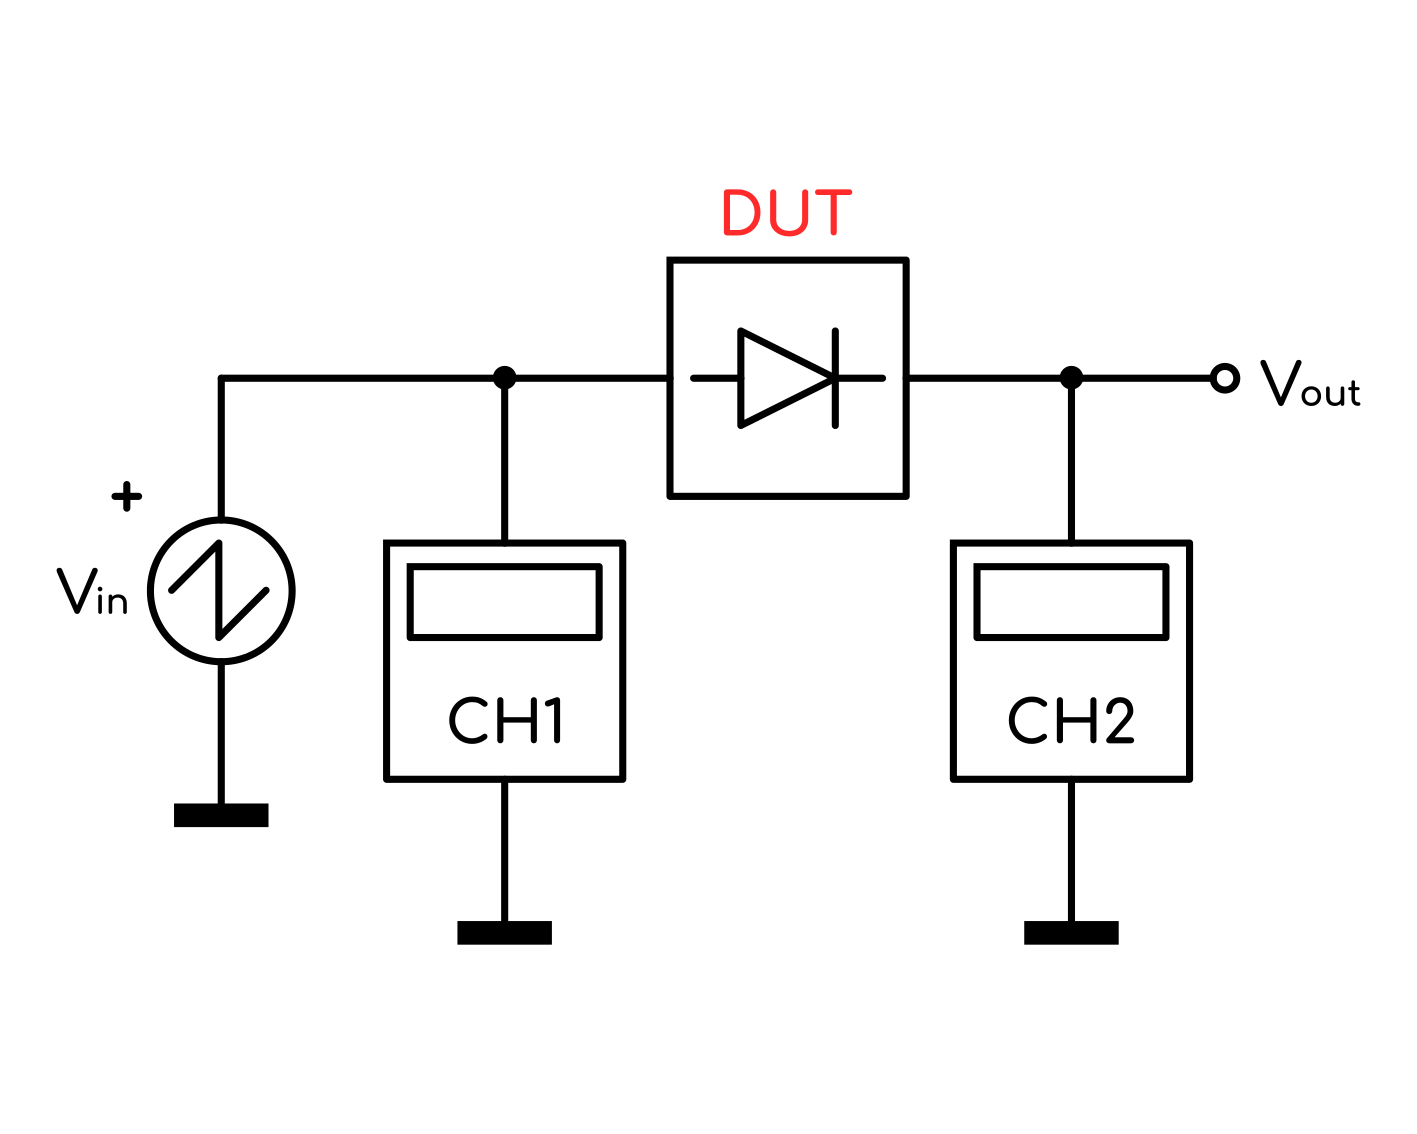
\includegraphics{block_diagrams/mis_clipper_oscilloscope.png}
        \caption{Setup di misura}
        \label{mis_clipper_oscilloscope}
    \end{subfigure}%
    \begin{subfigure}{.5\textwidth}
        \centering
        
\includegraphics{misc/oscilloscope_placeholder.png}
        \caption{Transcaratteristica}
        \label{clipper_transcharacteristic}
    \end{subfigure}

    \caption{Misura della transcaratteristica con oscilloscopio}
\end{figure}

\begin{figure}[H]
    \centering
    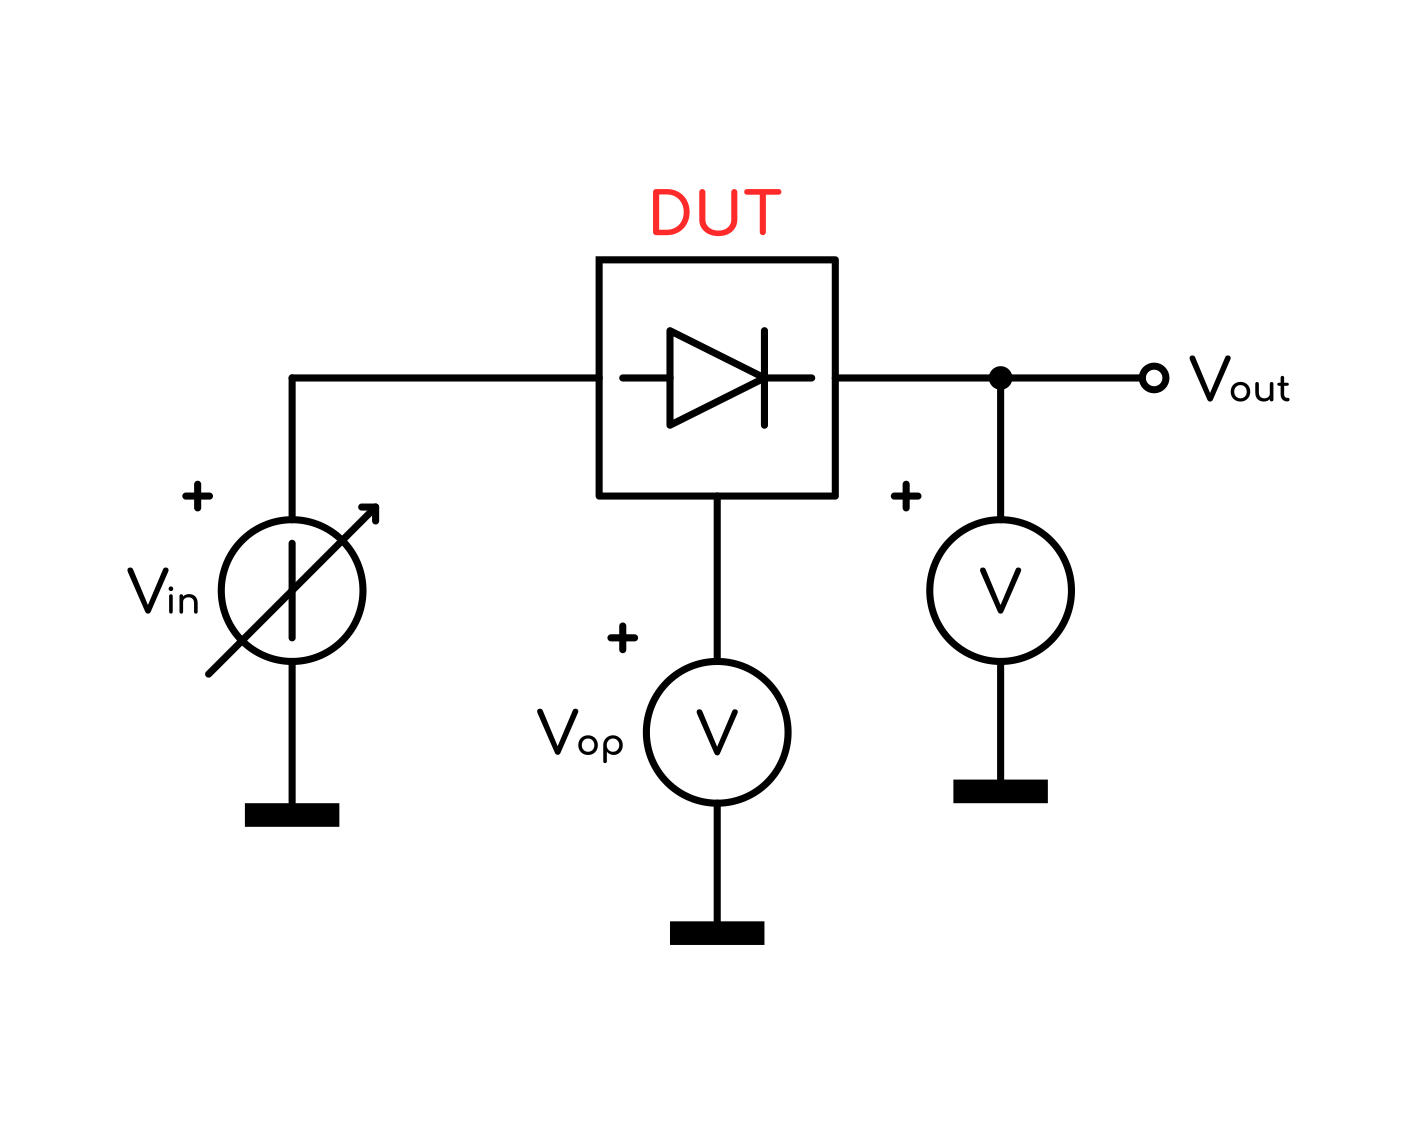
\includegraphics{block_diagrams/mis_clipper.png}
    \caption{Setup di misura}
    \label{mis_clipper}
\end{figure}

\begin{minipage}{0.45\textwidth}
    \centering
    \begin{table}[H]
        \centering
        \csvreader[
        tabular = |C||C|L|,
        table head = {\hline \rowcolor{myLightGrey} $V_{in}\ [V]$ & $V_{out}\ [V]$ & $V_{op}\ [V]$ \\\hline},
        late after line = \\\hline,
        ]{data/misure_clipper.csv}{}{
        \csvcoli & \csvcoliii & \csvcolv
        }
        \caption{Tabella dei dati raccolti}
        \label{clipper_table}
    \end{table}
\end{minipage}
\begin{minipage}{0.45\textwidth}
    \centering
    \begin{figure}[H]
        \centering
        \begin{tikzpicture}[scale = 0.85]
            \begin{axis}[
                    title = Transcaratteristica,
                    no marks,
                    xmin = -7, xmax = 7,
                    ymin = -7, ymax = 7,
                    grid = major,
                    grid style = {dashed, gray!30},
                    xlabel = $V_{in}$,
                    ylabel = $V_{out}$,
                    x unit = \si{\V}, y unit = \si{\V},
                    legend style = {at = {(0.5, -0.25)}, anchor = north},
                    cycle list name = modular,
                ]

                \addplot
                table[x = vin, y = vout attesa, col sep = comma]{./data/misure_clipper.csv};

                \addplot
                table[x = vin, y = vout misura, col sep = comma]{./data/misure_clipper.csv};

                \legend{Formula \ref{clipper_out}, Valori misurati}
            \end{axis}
        \end{tikzpicture}
    \end{figure}

    \begin{figure}[H]
        \begin{tikzpicture}[scale = 0.85]
            \begin{axis}[
                    title = Uscita all'operazionale,
                    no marks,
                    xmin = -7, xmax = 7,
                    ymin = -7, ymax = 12,
                    grid = major,
                    grid style = {dashed, gray!30},
                    xlabel = $V_{in}$,
                    ylabel = $V_{op}$,
                    x unit = \si{\V}, y unit = \si{\V},
                    legend style = {at = {(0.5, -0.25)}, anchor = north},
                    cycle list name = modular,
                ]

                \addplot
                table[x = vin, y = vop attesa, col sep = comma]{./data/misure_clipper.csv};

                \addplot
                table[x = vin, y = vop misura, col sep = comma]{./data/misure_clipper.csv};

                \legend{Formula \ref{clipper_op}, Valori misurati}
            \end{axis}
        \end{tikzpicture}
    \end{figure}
\end{minipage}

%--------------------------------------------------------------------------------------------
